%!TEX root = ../apese-rapport.tex
\section{Technologies utilisées}
	
	\subsection{Angular}
	Angular est un framework, écrit en TypeScript, succédant à AngularJS, son grand frère, qui lui a été écrit en JavaScript\cite{wikipedia-angularjs}. Il est développé par Google qui a décidé de le rendre libre et open source. \\
	Son but est de simplifier le développement d'applications et de pages web\cite{angular}. \\
	Nous l'avons utiliser afin de faire nos vues. Il est communément appelé \og{}Angular 2+\fg{} ou \og{}Angular 2\fg{}.
	
	\subsection{Docker}
	Docker est une société qui gère le mouvement des conteneurs et est aussi un logiciel libre qui automatise le déploiement d'applications dans des conteneurs logiciels. \\
	Il permet une véritable indépendance entre les applications, l'infrastructure, les développeurs et les opérations informatiques.\\ Il a été développé en Go.\cite{docker}\cite{wikipedia-docker}
	
	\subsection{Git}
	Git est un logiciel libre de gestion de versions décentralisé. \\
	Il a été conçu et développé par Linus Torvalds en 2005.\cite{wikipedia-git}
	
	\subsection{GitHub}
	GitHub est un service web d'hébergement et de gestion de développement de logiciels, utilisant Git. \\
	Nous l'avons utilisé afin de synchroniser notre travail, de l'organiser selon la méthode Agile ainsi que d'utiliser Travis CI.
	
	\subsection{Heroku}
	Heroku est un service de \og{}cloud computing\fg{} de type plate-forme en tant que service (PaaS). \\
	Celui-ci est utilisé comme modèle de déploiement d'applications Web. 
	Heroku Postgres est le service de base de données Cloud (DBaaaS) de Heroku basé sur PostgreSQL. Heroku Postgres offre des fonctionnalités telles que la protection continue, le rollback et la haute disponibilité.
	
	\subsection{OAuth}
	OAuth est un protocole libre qui permet d'accéder à des données tout en protégeant le pseudonyme et le mot de passe des utilisateurs. \\
	Nous avons utilisé la version 2 qui est la dernière à ce jour\cite{oauth2}\cite{wikipedia-oauth}. \\
	Nous avons choisi cette technologie pour gérer le token, car elle est fortement utilisée en entreprise et qu'elle est parfaitement intégrée avec le framework Spring.
	
	\subsection{Slack}
	Slack est une plateforme de collaboration et un logiciel de gestion de projets. \\
	Celle-ci sera utilisée dans le but de communiquer entre développeurs et avec le professeur. \\
	Elle nous permettra aussi de suivre les différents commits sur le dépôt GitHub grâce à son intégration native.
	
	\begin{figure}[ht]
		\centering
		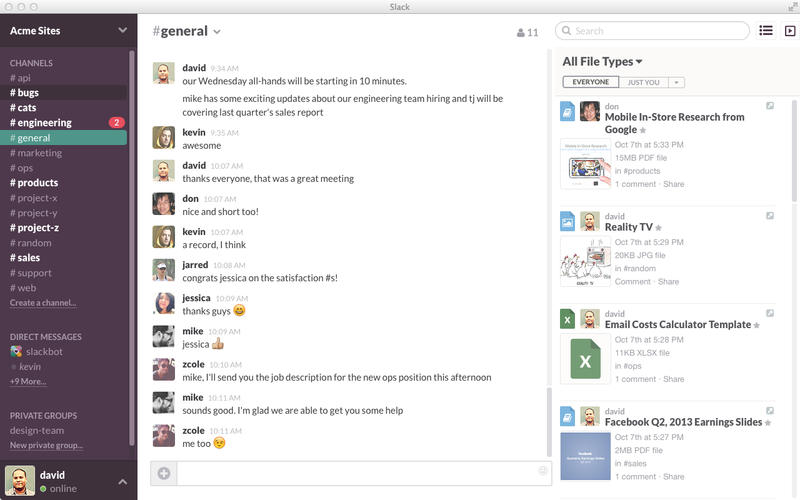
\includegraphics[width=0.85\textwidth]{slack-interface.jpg}
		\caption{Vue de la plateforme Slack}
	\end{figure}
	
	\subsection{Spring}
	Le framework libre Spring permet de construire et de définir l'infrastructure d'une application Java (back-end), dont il facilite le développement et les tests. \\
	Il s'agit d'une solution modulaire, ce qui en fait sa force et explique, avec sa richesse et son efficacité, l'engouement des développeurs pour ce framework. \\
	Le Java permet d'utiliser la programmation orientée objet.
	Du côté de la gestion des dépendances et de la compilation du site, nous avons utilisé le moteur de production Gradle.
	
	\subsection{Travis}
	Travis CI fournit un service en ligne utilisé pour compiler, tester et déployer le code source depuis, par exemple, GitHub. \\
	Dès qu'un commit est détecté sur une branche surveillée par Travis, celui-ci s'exécutera d'après la volonté du développeur. \\
	Le projet sera compilé, les tests seront lancés et le projet sera déployé sur Heroku si celui-ci lui est lié. \\
	L'état du projet dans Travis CI est toujours disponible et peut même être envoyé par mail.
	
	\subsection{TypeScript}
	TypeScript est un langage transcompilé libre et open-source développé par Microsoft. \\
	Nous n'avons pas eu le choix d'utiliser ce langage, car les versions d'Angular supérieure à la 2 ne fonctionne qu'avec lui.